\noindent V KiCadu byla vytvořena DPS pro DP 4. řádu, PP 2. řádu. Keramický kapacitor byl zvolen 561RTSQ10 (10 pF, jmenovité napětí stejnosměrného proudu 100 V). Jako zdroj proudu byl použit LM334 s přeladitelným odporem ve zpětné vazbě. Také lze použít PNP tranzistor, nebo operační zesilovač. Různé přístupy k řízení OTA vstupním proudem pomocí napěťového zdroje jsou popsány na obrázku \ref{s:DC} (literatura \cite{22}). Obrázek a) je nejjednodušší zapojení, ale toto zapojení je velmi citilivé na malé změny napětí. V zapojení b) je řídící napětí uzemněno, ale $V_c$ je citlivé na změny napětí mezi bází a emitorem tranzistoru a na úbytek napětí na diodě. V zapojení c) je řídící napětí také uzemněno a není závislé na součtu nebo vyrušení napětí na pn přechodech. Zenerova dioda je použita k udržení napětí. Frekvenční odezva OZ se zde neuvažuje, protože máme stejnosměrné napětí. Všechna zapojení jsou velmi citlivá na malé změny $V_c$.
\begin{figure}[h]
\centering
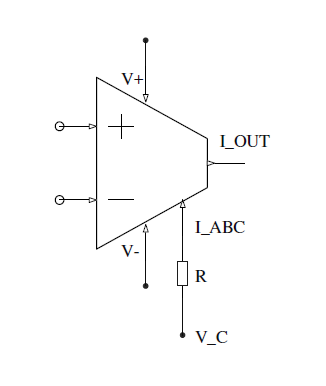
\includegraphics[scale=0.6]{current.png}
\caption{Schéma zapojení napěťového zdroje pro vstupní externí proud \label{s:DC} \cite{22}}
\end{figure}
\begin{figure}[h]
\centering
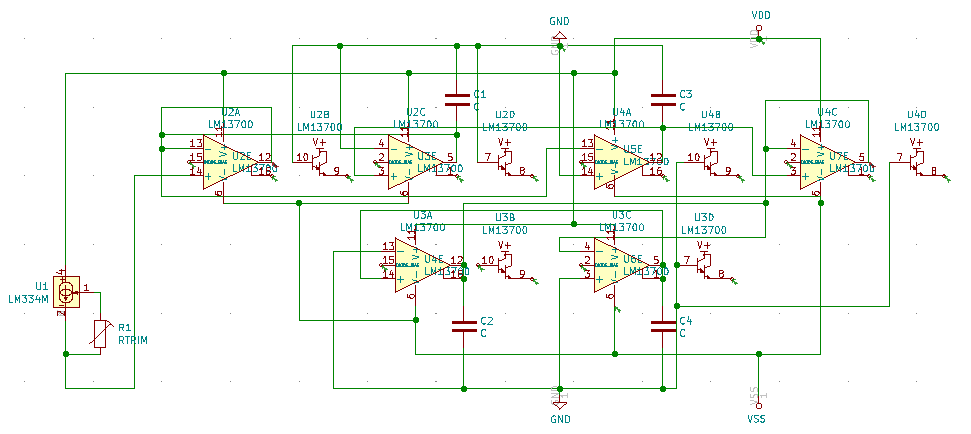
\includegraphics[scale=0.6]{kicad1.png}
\caption{Schéma obvodu v KiCadu}
\end{figure}